\chapter{最小割数量的敏感度分析}
\section{最小割数量的敏感度}
与此前工作不同的是,本文的近似最小割算法需要找到尽可多的解,
因此算法需要考虑输出的最小割数量,并确保隐私得到保护。
前文提到,图的差分隐私要求一条边的存在与否对输出的影响不能过大,
因此,图的最小割数量的敏感度的定量分析是必要的。
敏感度越大,需要添加的噪声也越大,
所以本掌将结合仙人掌图表示,将敏感度通过增加条件来限制在一个相对较小的值。

对于两个边相邻的图$G$和$G'$,不妨令$G'$的构造由在$G$中加入一条边权为$1$的边$(u,v)$完成。
在最小割数量计算函数的输入与输出都以适当的二进制形式进行编码的情况下,
最小割数量的敏感度为$d=|M_G-M_{G'}|$。

根据定理$\ref{the:mincutnumber}$,任意图$G$的最小割数量满足$1\leq M_G\leq n^2$,
因此可以得到一个平凡的结论$0\leq d\leq n^2$。
在不添加额外条件的情况下,该敏感度范围的最大值是可以取到的。


\begin{lemma}
  \label{lemma:mingganN}
  对于任意$n\geq 3$,存在图$G,G'$的构造方法,使得最小割数量的敏感度为$\Omega(n^2)$。
\end{lemma}
\begin{proof}
  为便于描述,首先将$G,G'$中的顶点编号,用$v_1$至$v_n$表示。
  令后文连接顶点所用的边的权重均为$x$。

  接下来给出$G,G'$的具体构造方法。
  在图$G$中,连接$v_1$与$v_2$,$v_2$与$v_n$,
  并对于所有整数$2\leq i<n$,连接$v_i$和$v_{i+1}$;
  图$G'$由在图$G$的基础上,增加一条连接$v_1$和$v_2$的边得到。
  图$G$由一个由$v_2,\dots,v_n$组成的$n-1$元环和一条边$(v_1,v_2)$构成,
  因此最小割值为$\Phi_G=x$,唯一的最小割是$(\{v_1\},V\backslash v_1)$,
  也就是是说,最小割数量$M_G=1$。
  图$G$由一个由$v_2,\dots,v_n$组成的$n-1$元环和$v_1,v_2$组成的$2$元环构成,
  因此最小割值$\Phi'_G=2x$,
  此时对于任意$2\leq i\leq j\leq n$,
  $(\{v_i,\ldots,v_j\},V\backslash \{v_i,\ldots,v_j\})$都是最小割的解,
  因此$M_{G'}=\frac{(n-1)(n-2)}2$。在这种构造方法下,$d=\Theta(n^2)$。
\end{proof}
\begin{figure}[htb]
    \centering
    \subfloat[图$G$]{
      \label{1}
      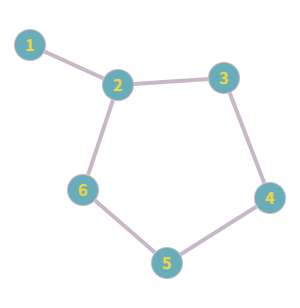
\includegraphics[height=5cm]{figures/graph001.png}}\hspace{4em}
    \subfloat[图$G'$]{
      \label{2}
      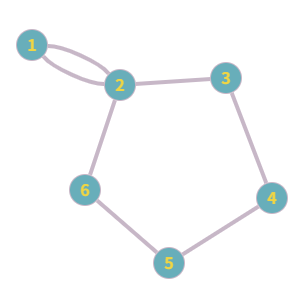
\includegraphics[height=5cm]{figures/graph002.png}}
    \caption{$n=6$时的构造示例}
    \label{fig:exA}
\end{figure}
图\ref{fig:exA}给出了一种$n=6$时的构造示例。
引理\ref{lemma:mingganN}表明,
边相邻图的最小割数量的敏感度较高
这意味着算法需要添加较大噪声,进而使得差分隐私下发布的最小割数量的可用性较低。
下一节,算法将引入额外约束条件并进行分析。
\section{约束条件下的敏感度}
给定图$G$,在加入一条单位边后,最小割的割值可能增加,也可能保持不变。
引理\ref{lemma:mingganN}指出,若图有一个割值为$x$的割和较多割值为$x+1$的割,
那么加边导致最小割的割值提高$1$后,会使最小割的数量出现较大的增幅。
因此,为了得到可用的结果,本节将加入额外限制条件,
使得边相邻图$G,G'$的最小割割值相同,
即图$G,G'$满足$\Phi_G=\Phi_{G'}$。
本节后续的分析将基于这一限制。

标准仙人掌图表示法包含了图所有最小割的信息,
因此其结构参数有助于加强对最小割数量敏感度分析的精细性。
对于图$G$以及其标准仙人掌图表示法$(\Gamma,\varphi)$,
本节引入以下参数来描述其结构:
\begin{itemize}
  % \item $\alpha_{n}$:图$G$的点数,即$|V_G|$%平均用的吧
  \item $\alpha_{g}$:标准仙人掌图表示法的点数,即$|V_{\Gamma}|$。
  \item $\alpha_{p}$:标准仙人掌图表示中所有点$v$对应的$|\varphi^{-1}(v)|$的最大值%平均用的吧
  \item $\alpha_{c}$:标准仙人掌图表示中环的数量。
  \item $\alpha_{r}$:标准仙人掌图表示中环长度的最大值。
  \item $\alpha_{d}$:标准仙人掌图表示中树结构的直径,也就是所有图上简单路径中,非环边数量的最大值。
  % \item $\beta_{p}$:图$G$的$p$割数量。
  % \item $\beta_{t}$:图$G$的$t$割数量。
\end{itemize}


前文提到,$G'$由在图$G$的基础上,增加一条边得到,记这条边为$(u,v)$。
边$(u,v)$在标准仙人掌图表示法$(\Gamma,\varphi)$中的位置
与最小割数量变化量有关,接下来给出具体分析。

若$\varphi(u)=\varphi(v)$,那么说明$u,v$之间不被任何最小割分隔开,
在仙人掌图表示法中,它们已经被视为连通性很高的两个点,
因此加入边$(u,v)$对最小割数量没有任何影响。

若$\varphi(u)\neq\varphi(v)$,记$U=\varphi(u)$,$V=\varphi(V)$。
标准仙人掌图表示法中的最小割分为两部分,
其中$p$割对应树表示的树边,
$t$割对应环上不相邻的边二元组。
$U$到$V$连边后,
树表示中$U$到$V$路径上的所有$p$割都将不再是最小割;
路径上所有$p$束对应的环代表的$t$割都会变少,
具体来说,对于一个$p$束$S$的环$G_S$,令$U\in x_{R'},V\in x_{R''}$,
所有将$x_{R'}$与$x_{R''}$分开的$t$割都将不再是最小割。

接下来对环上的情况进行定量分析。令$f(x)$为长度为$x$的环表示的$t$割数量,则
\begin{equation}
  f(x)=\begin{cases}
    \frac{x(x-3)}2&x\geq 3\\0&1\leq x\leq 2\end{cases}  
\end{equation}
假设环$G_S$的环长为$l$,$x_{R'}$与$x_{R''}$在环上的距离为$t$(满足$t\leq l-t$),
那么最小割的减少量为
\begin{equation}
  g(l,t)=f(l)-f(t)-f(l-t)-[t\geq 3]-[l-t\geq 3]
\end{equation}
令$G(l)=\max_{t=1}^{l-1}g(l,t)$,
其含义为长度为$l$的环对应的树结构顶点被路径$(U,V)$经过时,最小割减少量的最大值。
不妨对$l,t$的值进行讨论来得到该函数的取值:
当$1\leq l\leq 3$时,环上不包含$t$割,因此$G(l)=0$;
当$l=4$时,取$t=2$为极值,$G(4)=2$;
当$l\geq 5$时,$l-t\geq t$使得只需要考虑$[t\geq 3]$的两种取值,
即$t=1,t=2,t\geq 3$这三种情况。
\begin{itemize}
  \item 当$t=1$时,$g(l,1)\leq g(l,2)$,一定不优。
  \item 当$t=2$时,$g(l,2)=f(l)-f(l-2)-1=2l-6$;
  \item 当$t\geq 3$时,$g(l,t)=f(l)-f(t)-f(l-t)-2=-(t-\frac l2)^2+\frac{l^2}4-2$。
\end{itemize}
当$l=5$时,$t\leq 2$,因此$G(5)=g(5,2)=4$。
当$l\geq 6$时,$g(l,t)$在$t\geq 3$范围的极大值在$t=\left\lfloor\frac l2\right\rfloor$时取到,
且有$g(l,t)\geq g(l,2)$。综上,可以得到
\begin{equation}
  G(l)=\max{\{0,\lfloor\frac{l^2}4-2\rfloor\}}
\end{equation}

上述分析说明了加入一条边$(u,v)$在树结构图以及环上对最小割数量的影响。
这里还需要特别说明的是,
加入$(u,v)$使最小割的割值增加一的情况一定满足如下条件:
\begin{itemize}
  \item $\varphi(u)\neq\varphi(v)$。
  \item 标准仙人掌图表示法是一条链。
  \item $\varphi(u),\varphi(v)$分别是链的两个端点。
\end{itemize}
综上,在加入边不影响最小割值的情况下,最小割数量变化范围的表达式如下。

\begin{theorem}
    给定边相邻图$G,G'$,其中$G'$由在$G$中加入一条边权为$1$的边$(u,v)$得到。那么有
    \begin{equation}
      M_G-\alpha_d-\min{\{\alpha_d,\alpha_c,\frac{\alpha_g}{\alpha_r}\}}·\max{\{0,\lfloor\frac{\alpha_r^2}4-2\rfloor\}} \leq M_{G'}\leq M_G
    \end{equation}

\end{theorem}

这里链上的变化数量受到树结构图的直径约束,环上的变化数量受到路径经过环的数量以及每个环的环长约束。

最小割数量的变化还可以由$M_G$本身的值来进行更为简洁的估计。
前文提到,对于一个长度$l\geq 4$的环$G_S$,其表示的$t$割有$f(l)=\frac{l(l-3)}2$个,
边$(u,v)$经过它是会使其最小割数量减少至多$G(l)= \lfloor\frac{l^2}4-2\rfloor$。
此外,该$p$束$S$连接的不涉及$x_{R'},x_{R''}$的至少$l-2$条边对应的$p$割在加边后仍然为最小割。
因此,与该$p$束$S$相关的最小割的数量为$\frac{l^2-l-4}2$,减少量至多为$\lfloor\frac{l^2}4-2\rfloor$。
\begin{theorem}
  对于任意加边$(u,v)$,存在一种最小割分配方案,满足每个最小割至多分配至一个$p$束中,使得
  每个$p$束$S$损失的最小割数量不超过其分配量与$|G_S|$和的一半。
\end{theorem}

\begin{proof}
  按上文方法分配最小割后,$p$束$S$分配到的最小割数量为$\frac{l^2-l-4}2$,$G_S=l$
  其损失的最小割数量为$\lfloor\frac{l^2}4-2\rfloor$。有
  \begin{equation}
    \frac{l^2-l-4}2+l=\frac{l^2+l-4}2\geq \frac{l^2}2-4\geq 2\lfloor\frac{l^2}4-2\rfloor
  \end{equation}
\end{proof}
通过该方案,可以给出一个基于$M_G$的估计。

% 我们再给出最小割数量的估计
% \begin{theorem}
%   给定图$G$,有
%   \begin{equation}
%     \max{\{0,\frac{\alpha_r(\alpha_r-3)}2\}}+\alpha_d\leq M_G\leq \min{\{\alpha_c,\frac{\alpha_g}{\alpha_r}\}}·\max{\{0,\frac{\alpha_r(\alpha_r-3)}2\}}+\alpha_d
%   \end{equation}

% \end{theorem}
\begin{theorem}
  \label{sen}
  给定边相邻图$G,G'$,其中$G'$由在$G$中加入一条边权为$1$的边$(u,v)$得到。那么有
  \begin{equation}
    \frac{M_G}2-1.5n \leq M_{G'}\leq M_G
  \end{equation}

\end{theorem}
该定理给出了最小割数量敏感度的上界$\frac{M_G}2+1.5n$。
接下来将给出一个构造来说明这个上界可以近似地达到,
该构造下的最小割数量的敏感度与定理中最坏情况下的敏感度仅相差一个常乘法系数,
图$G$构造方法如下:
将$(1-\alpha) n$个点用边权$c$连成一条链,设链的两端分别为$v_1,v_2$;
将$\alpha n\geq 4$的点用边权$\frac c2$连成一个环,设环的一个对角线连接的两个点为$v_3,v_4$;
最后将$v_2,v_3$用边权为$c$的边相连,完成构造。

在该构造下,$M_G=(1-\alpha)n+\frac{\alpha n(\alpha n-3)}2$。敏感度最高的加边是$(v_1,v_4)$,
敏感度$M_G-M_{G'}=\lfloor\frac{\alpha^2 n^2}4\rfloor-2+(1-\alpha) n$。
取$\alpha=\frac 12$,可得$M_G=\frac{n(n-2)}8$,$M_G-M_{G'}=\lfloor\frac{n^2}{16}\rfloor-2+\frac 12n$。
在$n\geq 10$时有
\begin{equation}
  \frac{M_G}2+\frac32n= \frac{n^2}{16}+\frac{11}{8}n\leq 4(M_G-M_{G'})
\end{equation}


\section{平均敏感度}
前面的分析说明了,给定图$G$,
在最坏情况下,加入一条边带来的最小割数量变化较大,
也就是说敏感度较高。
这一节将通过平均敏感度,评估随机加边条件下,最小割数量变化较大的概率。

通常情况下,
平均敏感度定义中的边相邻图
会以图$G$与在其边集中删除一条边得到的图$G'$的形式给出。\cite{varma2023average}
但本节将采用加边的形式,
这能确保仙人掌图表示的结构易于分析。
以删边的形式定义平均敏感度,
可以估计一个图算法在规模较大的子图上的输出和完整图上的输出差异;
以加边的形式定义平均敏感度会在这一功能上有所欠缺,
但能与前文内容相结合,来给出最小割数量变化值的期望。

\begin{definition}
  图算法$A$的平均敏感度为
  \begin{equation}
    \mathbb E_{e\in V^2,\Phi(G)=\Phi((V,E\cup\{e\}))}[d_{Ham}(A(G),A((V,E\cup\{e\})))]
  \end{equation}
\end{definition}

接下来,本文将给出一种$G$的构造来说明,
随机加边条件下,最小割数量的变化的平均值可以取到一个较高的值。
记$W(n)$为规模为$n$的图的最高敏感度,具体构造步骤如下:
首先生成一个规模为$\frac 13n$的图$G_t$,
使得$G_t$在加入边$(u,v)$时得到该规模下最高的敏感度$W(\frac 13n)$;
接下来令$\frac 13n$个点与$u$用极大的边权相连,令另外$\frac 13n$个点与$v$用极大的边权相连。
以该方法构造出的图$G$中,$u,v$分别与$\frac 13n$个点紧密相连,
这意味着当选取的边的两端分别位于这两个点集时,
其产生的最小割数量的变化等价与边$(u,v)$。

因此,在该构造下最小割数量函数$M$的平均敏感度满足
\begin{equation}
  \mathbb E_{e\in V^2,\Phi(G)=\Phi(G+e)}[d_{Ham}(M(G),M(G+e))]\geq \frac{\frac 13n(\frac 13n-1)}{n(n-1)}W(\frac 13n)
\end{equation}
最高敏感度$W$是一个$n$的二次多项式。综上,存在一个常数$\beta$使得在该构造下
\begin{equation}
  \mathbb E_{e\in V^2,\Phi(G)=\Phi(G+e)}[d_{Ham}(M(G),M(G+e))]\geq \beta W(n)
\end{equation}
分析表明,随机加边条件下,最小割数量的变化可以取到一个较高的期望。